\documentclass{article}

\newcommand{\thistitle}{Introduction to Modern C++ Course Outline}
\newcommand{\me}{Ryan Baker}

\usepackage{hyperref}
\usepackage[dvipsnames]{xcolor}
\usepackage{listings}

\title{\thistitle}
\author{\me}
\date{\today}

\definecolor{JadeGreen}{RGB}{91,158,62}
\definecolor{LightGray}{RGB}{247,247,247}
\lstdefinestyle{catppuccin}{
	backgroundcolor=\color{LightGray},
    commentstyle=\color{CadetBlue},
	numberstyle=\footnotesize\ttfamily\color{Gray},
	stringstyle=\color{JadeGreen},
	keywordstyle=\color{BurntOrange},
	basicstyle=\ttfamily\color{Black},
	breakatwhitespace=true,
	breaklines=true,
	captionpos=b,
	keepspaces=true,
	numbers=left,
	numbersep=5pt,
	showspaces=false,
	showstringspaces=false,
	showtabs=false,
	tabsize=4,
    frame=single,
    xleftmargin=10pt,
    xrightmargin=10pt,
    aboveskip=10pt,
    belowskip=10pt,
    framexleftmargin=10pt,
    framexrightmargin=10pt,
    framesep=5pt,
    rulecolor=\color{Gray},
}

\lstset{style=catppuccin}

\hypersetup{
	colorlinks=true,
	hidelinks=false,
	linkcolor=RoyalBlue,
	citecolor=ForestGreen,
	filecolor=DarkOrchid,
	urlcolor=BurntOrange,
	runcolor=BrickRed,
    pdftitle={\thistitle},
	pdfauthor={\me},
}

\newcommand{\inlinecpp}[1]{\lstinline[language=C++]|#1|}
\newcommand{\centercpp}[1]{\begin{center}\lstinline[language=C++]|#1|\end{center}}
\newcommand{\inputcpp}[1]{\lstinputlisting[language=C++]{#1}}

\newcommand{\titleone}{Introduction and Setup}
\newcommand{\titletwo}{C++ Programming Basics}
\newcommand{\titlethree}{How C++ Works}
\newcommand{\titlefour}{Introduction to OOP}
\newcommand{\titlefive}{Advanced OOP}
\newcommand{\titlesix}{Templates}
\newcommand{\titleseven}{The C++ Standard Library}
\newcommand{\titleeight}{Safety in C++}
\newcommand{\titlenine}{Compile-Time Programming}


\title{\thistitle}
\author{\me}
\date{\today}

\begin{document}

\maketitle
\pagebreak

\centering
\section*{Week 1: \titleone}
\documentclass{article}

\newcommand{\titleone}{Introduction and Setup}
\newcommand{\titletwo}{C++ Programming Basics}
\newcommand{\titlethree}{How C++ Works}
\newcommand{\titlefour}{Introduction to OOP}
\newcommand{\titlefive}{Advanced OOP}
\newcommand{\titlesix}{Templates}
\newcommand{\titleseven}{The C++ Standard Library}
\newcommand{\titleeight}{Safety in C++}
\newcommand{\titlenine}{Compile-Time Programming}

\newcommand{\thistitle}{\titleone}
\newcommand{\me}{Ryan Baker}

\usepackage{hyperref}
\usepackage[dvipsnames]{xcolor}
\usepackage{listings}

\title{\thistitle}
\author{\me}
\date{\today}

\definecolor{JadeGreen}{RGB}{91,158,62}
\definecolor{LightGray}{RGB}{247,247,247}
\lstdefinestyle{catppuccin}{
	backgroundcolor=\color{LightGray},
    commentstyle=\color{CadetBlue},
	numberstyle=\footnotesize\ttfamily\color{Gray},
	stringstyle=\color{JadeGreen},
	keywordstyle=\color{BurntOrange},
	basicstyle=\ttfamily\color{Black},
	breakatwhitespace=true,
	breaklines=true,
	captionpos=b,
	keepspaces=true,
	numbers=left,
	numbersep=5pt,
	showspaces=false,
	showstringspaces=false,
	showtabs=false,
	tabsize=4,
    frame=single,
    xleftmargin=10pt,
    xrightmargin=10pt,
    aboveskip=10pt,
    belowskip=10pt,
    framexleftmargin=10pt,
    framexrightmargin=10pt,
    framesep=5pt,
    rulecolor=\color{Gray},
}

\lstset{style=catppuccin}

\hypersetup{
	colorlinks=true,
	hidelinks=false,
	linkcolor=RoyalBlue,
	citecolor=ForestGreen,
	filecolor=DarkOrchid,
	urlcolor=BurntOrange,
	runcolor=BrickRed,
    pdftitle={\thistitle},
	pdfauthor={\me},
}

\newcommand{\inlinecpp}[1]{\lstinline[language=C++]|#1|}
\newcommand{\centercpp}[1]{\begin{center}\lstinline[language=C++]|#1|\end{center}}
\newcommand{\inputcpp}[1]{\lstinputlisting[language=C++]{#1}}


\title{\thistitle}
\author{\me}
\date{\today}

\begin{document}

\maketitle
\tableofcontents

\section{Course Introduction}

\subsection{Overview of Lecture Series}

\section{Features of C++}

\subsection{Evolution of C++}

\noindent
C++ was developed in 1979 by Bjarne Stroustrup as a simple extension of C. Since then, it has evolved into a modern multi-paradigm language with major updates every three years (C++26 is on its way). Each update introduces features for better performance, safety, flexibility, and developer experience. 

\subsection{The C++ Philosophy}

\noindent
C++ is a sharp tool. It prioritizes manual control over all else, allowing for direct memory manipulation and fine-grained resource management. The philosophy is to give the developer the tools for flexibility and performance, but with the responsibility to manage complexity.

\subsection{C++ vs. Other Languages}

\paragraph{Compiled vs. Interpreted}
C++ is a \textit{compiled} language, meaning the source code is translated into machine code before it is executed. This allows for a faster run time and more control over hardware aspects. This contrasts with \textit{interpreted} languages, like Python, translated and executed line by line. Interpreted languages tend to be quicker to develop and easier to use.

\paragraph{Strongly Typed}
Strongly typed languages, such as C++, require the explicit specification of datatypes and enforce type assignments at compile and run time. This makes it harder to make type mistakes and promotes code stability.

\paragraph{Multi-Paridigm}
A programming paradigm is a high-level way to structure and conceptualize your program. Some languages enforce a certain paradigm, such as procedural programming or object-oriented programming, but not C++. C++ supports multiple programming paradigms, awarding more freedom to the programmer.

\section{Environment Setup}

\subsection{Tools Required}

\noindent
To develop C++, you need two basic tools: a \textbf{text editor} and a \textbf{compiler}.

\subsubsection{Text Editor}

\begin{itemize}
	\item What is a text editor? A tool at edits text. \inlinecpp{// duh}
	\item \textbf{Text Editor vs. IDE:} A text editor is a basic tool for writing plain text, while an IDE (Integrated Development Environment) is a more comprehensive tool that includes a code editor, debugging tools, code completion, an build automation.
	\item Some popular text editors include:
	\begin{itemize}
		\item \textbf{Visual Studio Code:} A free, open-source IDE with support for C++ through extensions.
		\item \textbf{CLion:} An IDE specifically built for C++ with advanced features.
		\item \textbf{Vim/Neovim:} My personal choice. Has a steep learning curve, but absolutely worth it.
		\begin{itemize}
			\item If you decide to go with Vim or Neovim, I recommend spending some time configuring your setup. Feel free to ask me for help.
		\end{itemize}
	\end{itemize}
\end{itemize}

\subsubsection{Compiler}

\begin{itemize}
	\item \textbf{Definition:} The compiler converts your C++ source code into machine-readable instructions.
	\item Common C++ compilers include:
	\begin{itemize}
		\item \textbf{gcc:} The GNU Compiler Collection, a popular open-source compiler. Best for Windows OS and Linux.
		\item \textbf{clang:} My personal favorite, known for its performance and diagnostics. Best for Mac OS.
		\item \textbf{MSVC:} An increasingly irrelevant piece of garbage. Second best for Windows.
	\end{itemize}
	\item Throughout the lecture series, I will be using \texttt{clang}. If a certain \texttt{clang} flag or directive does not work for your compiler, simply look up its equivalent.
\end{itemize}

\subsection{``Hello, World!'' Example}

\noindent
With your text editor of choice, write the following C++ program:

\begin{lstlisting}[language=C++]
#include <iostream>

int main()
{
	std::cout << "Hello, World!" << std::endl;
	return 0;
}
\end{lstlisting}

\noindent
Compile and run the program with your compiler of choice. You should see ``Hello, World!'' printed to the console.

\section{Basic Syntax and Structure}

\subsection{Basic Structure of a C++ Program}

\subsubsection{\inlinecpp{int main()}}

\begin{itemize}
	\item \textbf{Entry Point:} The \inlinecpp{main()} function is where every C++ program starts executing. It serves as the ``entry point'' for a program.
	\item \textbf{Return Value:} \inlinecpp{main()} returns an integer to indicate the program's exit status. By convention, returning \inlinecpp{0} means successful execution.
	\begin{itemize}
		\item In modern C++, \inlinecpp{return 0} is implicit
	\end{itemize}
\end{itemize}

\begin{lstlisting}[language=C++]
int main() {} // the shortest complete C++ program
\end{lstlisting}

\subsection{Foundational Concepts}

\subsubsection{Semicolons, \inlinecpp{/* comments */}, and Whitespace}

\begin{itemize}
	\item \textbf{Semicolons:} Every statement in C++ ends with a semicolon:
	\centercpp{std::cout << "Hello, World!" << std::endl;}
	\begin{itemize}
		\item This lets the compiler know that the line is finished
	\end{itemize}
	\item \textbf{Comments:} Comments are a way of ``taking notes'' within your code. They are ignored by the compiler entirely, but help you and other developers understand the code.
	\item There are two ways of writing comments:
	\begin{itemize}
		\item \textbf{Single Line:} Single line comments are prefixed with \inlinecpp{//}:
		\centercpp{int main() // main function serves as the entry point}
		\item \textbf{Block:} Block comments are written with \inlinecpp{/* */} notation:
		\centercpp{int /* why is there a comment here? */ main()}
		\item \textsl{Ryan's Advice:} Lightly prefer \inlinecpp{//} to \inlinecpp{/* */} because the parsing of \inlinecpp{/* */} is more complicated and can lead to errors if you aren't careful.
	\end{itemize}
	\item \textbf{Whitespace:} C++ could not care less about whitespace. Whitespace includes spaces, tabs, and newlines.
	\begin{itemize}
		\item This means that is its possible, although not generally recommended, to write a C++ program in one line of code:
	\end{itemize}
	\centercpp{int main() \{ std::cout << "Hello, World!" << std::endl; \}}
\end{itemize}

\subsubsection{Line-by-Line Execution}

\noindent
In C++, the program executes statement sequentially, starting from the top of \inlinecpp{main()} and moving downward.

\begin{lstlisting}[language=C++]
int main()
{
	std::cout << "First"  << std::endl;  // guaranteed
	std::cout << "Second" << std::endl;  // to print
	std::cout << "Third"  << std::endl;  // in order
}
\end{lstlisting}

\subsection{Input and Output}

\section{Datatypes and Variables}

\subsection{Primitive Types}

\subsubsection{\inlinecpp{int}, \inlinecpp{char}, \inlinecpp{bool}, \inlinecpp{float}, \inlinecpp{void}} 

\noindent
When we're programming, all we are really doing is manipulating data. Data comes in many forms, shapes, and sizes, together forming a \textit{datatype}. C++ has several built-in datatypes, called primitive types:

\begin{itemize}
	\item[\textcolor{BurntOrange}{\texttt{int}}:] Used to store integer values (e.g., 5, -10, 42)
	\begin{itemize}
		\item Integers can be \textit{signed} (represent $\pm$) or \textit{unsigned} (only positive).		
		\item Because a computer's memory is finite, so too is the range of an \inlinecpp{int}.
		\begin{itemize}
			\item The maximum value of an unsigned \inlinecpp{int} can be calculated as $2^w$ where $w$ is the width of the \inlinecpp{int} in bits. The minimum is 0.
			\begin{itemize}
				\item The range of a \inlinecpp{uint32_t} is $[0, 2^{32}-1]=[0, 4294967295]$
			\end{itemize}
			\item For signed integers, the maximum value is $2^{w-1}-1$ and the minimum value is $-2^{w-1}$ where $w$ is the width in bits.
			\begin{itemize}
				\item The range of an \inlinecpp{int32_t} is $[-2147483648, 2147483647]$
			\end{itemize}
		\end{itemize}
	\end{itemize}
	\item[\textcolor{BurntOrange}{\texttt{char}}:] Used to store single characters (e.g., `a', `2')
	\begin{itemize}
		\item Characters are just integers in disguise. Every character has a corresponding integer value according to the \textbf{ASCII Table}.
		\centercpp{std::cout << int('a') << std::endl; // 97}
		\centercpp{std::cout << char(97) << std::endl; // `a'}
	\end{itemize}
	\item[\textcolor{BurntOrange}{\texttt{bool}}:] 
	\item[\textcolor{BurntOrange}{\texttt{float}}:] 
	\item[\textcolor{BurntOrange}{\texttt{void}}:] 
\end{itemize}

\subsubsection{\inlinecpp{sizeof} Operator}

\subsection{Declaration and Definition}

\subsubsection{Assignment Operator \inlinecpp{=}}

\subsubsection{Brace Initialization \inlinecpp{\{\}}}

\subsection{Arithmetic Operators}

\end{document}

\pagebreak

\centering
\section*{Week 2: \titletwo}
\documentclass{article}

\newcommand{\titleone}{Introduction and Setup}
\newcommand{\titletwo}{C++ Programming Basics}
\newcommand{\titlethree}{How C++ Works}
\newcommand{\titlefour}{Introduction to OOP}
\newcommand{\titlefive}{Advanced OOP}
\newcommand{\titlesix}{Templates}
\newcommand{\titleseven}{The C++ Standard Library}
\newcommand{\titleeight}{Safety in C++}
\newcommand{\titlenine}{Compile-Time Programming}

\newcommand{\thistitle}{\titletwo}
\newcommand{\me}{Ryan Baker}

\usepackage{hyperref}
\usepackage[dvipsnames]{xcolor}
\usepackage{listings}

\title{\thistitle}
\author{\me}
\date{\today}

\definecolor{JadeGreen}{RGB}{91,158,62}
\definecolor{LightGray}{RGB}{247,247,247}
\lstdefinestyle{catppuccin}{
	backgroundcolor=\color{LightGray},
    commentstyle=\color{CadetBlue},
	numberstyle=\footnotesize\ttfamily\color{Gray},
	stringstyle=\color{JadeGreen},
	keywordstyle=\color{BurntOrange},
	basicstyle=\ttfamily\color{Black},
	breakatwhitespace=true,
	breaklines=true,
	captionpos=b,
	keepspaces=true,
	numbers=left,
	numbersep=5pt,
	showspaces=false,
	showstringspaces=false,
	showtabs=false,
	tabsize=4,
    frame=single,
    xleftmargin=10pt,
    xrightmargin=10pt,
    aboveskip=10pt,
    belowskip=10pt,
    framexleftmargin=10pt,
    framexrightmargin=10pt,
    framesep=5pt,
    rulecolor=\color{Gray},
}

\lstset{style=catppuccin}

\hypersetup{
	colorlinks=true,
	hidelinks=false,
	linkcolor=RoyalBlue,
	citecolor=ForestGreen,
	filecolor=DarkOrchid,
	urlcolor=BurntOrange,
	runcolor=BrickRed,
    pdftitle={\thistitle},
	pdfauthor={\me},
}

\newcommand{\inlinecpp}[1]{\lstinline[language=C++]|#1|}
\newcommand{\centercpp}[1]{\begin{center}\lstinline[language=C++]|#1|\end{center}}
\newcommand{\inputcpp}[1]{\lstinputlisting[language=C++]{#1}}


\title{\thistitle}
\author{\me}
\date{\today}

\begin{document}

\maketitle
\tableofcontents
\pagebreak

\section{The Build Process}

\subsection{Source Code}

\subsection{Preprocessor}

\subsubsection{Text Substitution}

\subsubsection{Conditional Compilation}

\subsubsection{File Inclusion}

\subsubsection{Preprocessor Output}

\subsection{Compilation}

\subsubsection{Compiler Output}

\subsection{Linking}

\section{Introduction to Memory}

\subsection{How C++ Uses Memory}

\subsection{Pointers}

\subsubsection{\inlinecpp{NULL} Pointers}

\subsubsection{Pointer Arithmetic}

\subsubsection{Pointers to Pointers}

\section{Memory Layout}

\subsection{Text Segment}

\subsection{Static Memory}

\subsubsection{Variable Lifetime}

\subsection{The Heap}

\subsubsection{Operators \inlinecpp{new} and \inlinecpp{delete}}

\subsubsection{Memory Leaks}

\subsection{The Stack}

\subsubsection{The Stack Pointer}

\end{document}

\pagebreak

\centering
\section*{Week 3: \titlethree}
\documentclass{article}

\usepackage{hyperref}
\usepackage[dvipsnames]{xcolor}
\usepackage{listings}
\usepackage{amsmath}
\usepackage{tikz}

\title{C++: From Code to Execution
}
\author{Ryan Baker}
\date{\today}

\definecolor{JadeGreen}{RGB}{91,158,62}
\lstdefinestyle{catppuccin}{
	backgroundcolor=\color{White},
	commentstyle=\color{Gray},
	numberstyle=\footnotesize\ttfamily\color{Gray},
	stringstyle=\color{JadeGreen},
	keywordstyle=\color{BurntOrange},
	basicstyle=\ttfamily\footnotesize\color{Black},
	breakatwhitespace=false,
	breaklines=true,
	captionpos=b,
	keepspaces=true,
	numbers=left,
	numbersep=5pt,
	showspaces=false,
	showstringspaces=false,
	showtabs=false,
	tabsize=4,
}
\lstset{style=catppuccin}

\hypersetup{
	colorlinks=true,
	hidelinks=false,
	linkcolor=RoyalBlue,
	citecolor=ForestGreen,
	filecolor=DarkOrchid,
	urlcolor=BurntOrange,
	runcolor=BrickRed,
	pdftitle={C++: From Code to Execution},
	pdfauthor={Ryan Baker},
}

\begin{document}

\maketitle
\tableofcontents
\pagebreak

\subsection*{Lecture Objectives}

\noindent By the end of this lecture, you should:
\begin{itemize}
	\item Understand pointers, references, and indirection
	\item Be able to use arrays to store and manipulate many variables
	\item Be able to reason about memory segments, and how they effect execution
\end{itemize}

\section{Pointers}

\noindent
Computers work with memory. Everything, from variables, to functions, to the actual machine code itself is stored in memory. Memory is extremely important. Pointers are tools to accessing and manipulating memory.

\subsection{Basics of Pointers}

\begin{itemize}
	\item What is a pointer?
	\begin{itemize}
		\item A pointer is a variable (an integer) that represents a memory address
	\end{itemize}
	\item Why use pointers? Pointer provide:
	\begin{itemize}
		\item Dynamic memory allocation and deallocation
		\item Passing large objects efficiently to functions
		\item Manipulation of memory at a low-level
	\end{itemize}
	\item Pointer syntax: \texttt{<type>* <name>}
	\begin{itemize}
		\item \textbf{Example:} \texttt{int* ptr;} declares a pointer to an \texttt{int}
		\item \textbf{Example:} \texttt{int* ptr = nullptr;} declares a \texttt{NULL} pointer to an \texttt{int}
		\begin{itemize}
			\item \texttt{nullptr} is a keyword that represents a null pointer value
			\item \texttt{NULL} is a pointer value that points to address 0 (invalid)
		\end{itemize}
	\end{itemize}
	\item Using pointers:
	\begin{itemize}
		\item Address-of operator: \texttt{\&}
		\begin{itemize}
			\item Use the address-of operator in front of a variable to get its address
			\item \texttt{std::cout << \&x << std::endl;} prints the address of \texttt{x}
			\item \texttt{int* ptr = \&x;} sets the value of \texttt{ptr} to the address of \texttt{x}
		\end{itemize}
		\item Dereference operator: \texttt{*}
		\begin{itemize}
			\item Use the dereference operator in front of a pointer to get the value
			\item \texttt{std::cout << *ptr << std::endl;} prints the value pointed to
			\item \texttt{int x = *ptr;} sets the value of \texttt{x} to the the memory pointed to by \texttt{ptr}
		\end{itemize}
		\item Together, the address-of and dereference operators allow you to access and manipulate memory with pointers
	\end{itemize}
\end{itemize}

\lstinputlisting[language=C++]{code/pointer.cpp}

\subsection{Pointer Arithmetic}

\begin{itemize}
	\item What is pointer arithmetic?
	\begin{itemize}
		\item Pointer arithmetic involves performing operations (such as addition or subtraction) on pointer variables, adjusting the memory address they reference based on the size of the data type they point to.
	\end{itemize}
	\item Pointer arithmetic in action:
	\lstinputlisting[language=C++]{code/parithmetic.cpp}
	\item \textbf{Key point:} Pointer arithmetic on \texttt{void*}s causes errors because \texttt{sizeof(void)} is undefined
\end{itemize}

\subsection{Pointers to Pointers}

\begin{itemize}
	\item Pointers are variables that represent memory addresses of other variables
	\item This means that a pointer can ``point to'' another pointer
	\begin{itemize}
		\item \texttt{sizeof(<pointer>)} = 8 (usually, for 64-bit systems)
		\begin{itemize}
			\item If you're working on a 32-bit system: \texttt{sizeof(<pointer>)} = 4
		\end{itemize}
	\end{itemize}
	\lstinputlisting[language=C++]{code/ptop.cpp}
\end{itemize}

\section{References}

\noindent
Every reference is just a pointer in disguise. They exist to help make working with pointers a bit easier.

\begin{itemize}
	\item What is a reference?
	\begin{itemize}
		\item A reference is a way to ``reference'' an existing variable
		\item There is no such thing as a \texttt{NULL} reference
		\item Think of references as aliases
	\end{itemize}
	\item Reference syntax: \texttt{<type>\& <name> = <variable>}
	\begin{itemize}
		\item \textbf{Example:} \texttt{int\& ref = x;} ``refers'' \texttt{ref} to \texttt{x}
	\end{itemize}
	\lstinputlisting[language=C++]{code/reference.cpp}
	\item\textbf{Example:} \texttt{increment(int x) \{...\}} vs. \texttt{increment(int\& x) \{...\}}
	\begin{itemize}
		\item When you pass by reference, the original value is modified
		\item When you pass by value (not reference), the original is untouched
	\end{itemize}
\end{itemize}

\section{Arrays}

\begin{itemize}
	\item What is an array?
	\begin{itemize}
		\item An array is a collection of variables stored contiguously
		\item Truly, an array is simply a pointer to its first element
	\end{itemize}
	\item When to use arrays?
	\begin{itemize}
		\item We often need to represent an entire collection of data, rather than creating many many variables, we can create an array
		\item \textbf{Example:} To represent the squares of a chess board, I could either create 64 variables: \texttt{int a1, int b1, ... int h8}, or use an array
	\end{itemize}
	\item Array syntax: \texttt{<type> <name>[<size>] = \{...\}}
	\begin{itemize}
		\item \textbf{Example:} \texttt{int chess\_board[64];}
	\end{itemize}
	\item Using arrays: \texttt{<name>[<index>]}
	\begin{itemize}
		\item Indices start at 0
		\item \textbf{Example:} \texttt{int square = chess\_board[32];}
		\item The square bracket (access) operator \texttt{[]} expands to a dereference:
		\begin{itemize}
			\item \texttt{arr[5]} $\rightarrow$ \texttt{*(arr + 5)} (Recall pointer arithmetic)
			\item This is why indices begin at 0
			\item To prove this: \texttt{arr[5] == 5[arr]}
		\end{itemize}
	\end{itemize}
	\lstinputlisting[language=c++]{code/access.cpp}
\end{itemize}

\section{Memory Segments}

\noindent
The memory that your operating system assigns to your executable is split up into different segments. Each segment is designed to hold a different type of data.

\begin{center}
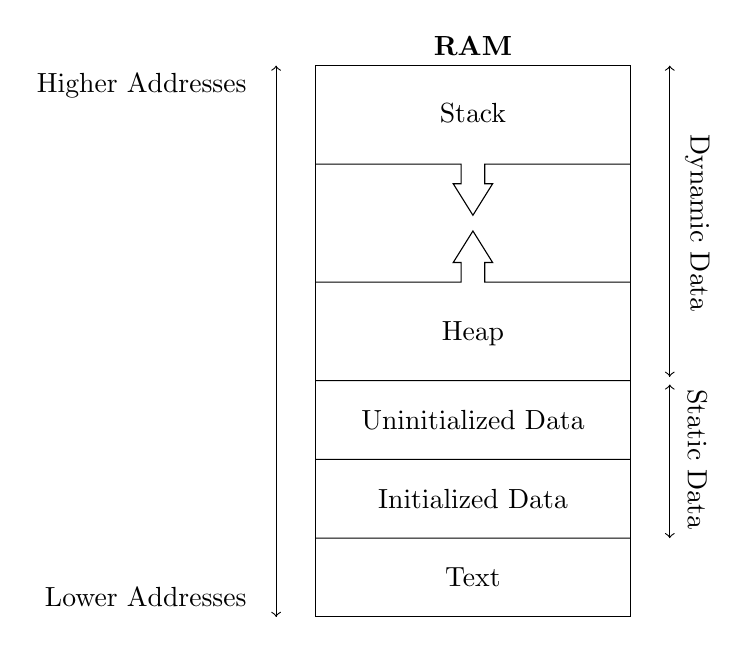
\begin{tikzpicture}

\draw
(0,0) -- ++(4,0) -- ++(0,7) -- ++(-4,0) -- (0,0)
;
\draw[->](-0.5,0) -- (-0.5,7);
\draw[->](-0.5,7) -- (-0.5,0);
\draw
(-0.75,6.75) node[left] {Higher Addresses}
(-0.75,0.25) node[left] {Lower Addresses}
(2,7) node[above] {\textbf{RAM}}
(0,1) -- (4,1) (2,0.5) node[] {Text}
(0,2) -- (4,2) (2,1.5) node[] {Initialized Data}
(0,3) -- (4,3) (2,2.5) node[] {Uninitialized Data}
(0,4.25) -- ++(1.85,0) -- ++(0,0.25) -- ++(-0.1,0) -- ++ (0.25,0.4) -- ++(0.25,-0.4) -- ++(-0.1,0) -- ++(0,-0.25) -- ++(1.85,0)
(0,5.75) -- ++(1.85,0) -- ++(0,-0.25) -- ++(-0.1,0) -- ++ (0.25,-0.4) -- ++(0.25,0.4) -- ++(-0.1,0) -- ++(0,0.25) -- ++(1.85,0)
(2,3.6) node[] {Heap}
(2,6.4) node[] {Stack}
;
\draw[->] (4.5,1)--(4.5,2.95) ;
\draw[->] (4.5,2.95)--(4.5,1) ;
\draw[->] (4.5,3.05) --(4.5,7);
\draw[->] (4.5,7) --(4.5,3.05);
\draw
(4.85,5) node[rotate=-90] {Dynamic Data}
(4.85,2) node[rotate=-90] {Static Data}
;
\end{tikzpicture}
\end{center}

\subsection{Text Segment}

\noindent
The text segment, a.k.a. the ``code'' segment, contains the machine code instructions to run your program. It is fixed in size and read-only. It also contains integer and string literals present in your code.

\subsection{Static Memory}

\noindent
Static memory is allocated at compile time and read directly from the executable. It contains global and static variables. This segment is divided into \textit{initialized} and \textit{uninitialized} data. The only difference is whether or not the variable has a compile-time initialized value.

\subsection{Heap Memory}

\begin{itemize}
	\item What is the heap?
	\begin{itemize}
		\item The heap is a memory segment that is variable in size and used for dynamic memory allocation.
        \item It gives the programmer direct control over memory, allowing you to allocate and deallocate memory manually.
        \item Think of it as a large pool of memory available for your program's use (though the term ``heap'' doesn't refer to this).
	\end{itemize}
	\item How to use the heap?
	\begin{itemize}
		\item Use the \texttt{new} operator to allocate memory:
		\begin{itemize}
		\item \texttt{int* ptr = new int(42);} Allocates an \texttt{int} with value 42
		\end{itemize}
		\item Use the \texttt{delete} operator to free memory:
		\begin{itemize}
		\item \texttt{delete ptr;} Frees the memory allocated to \texttt{ptr}
		\end{itemize}
	\end{itemize}
	\lstinputlisting[language=C++]{code/heap.cpp}
	\item \textbf{Memory leaks:}
	\begin{itemize}
		\item A memory leak occurs when memory is allocated on the heap but never freed, causing the program to consume more memory over time.
		\item Forgetting to deallocate memory with \texttt{delete} leads to memory leaks
		\item Dereferencing pointers that have been deleted is undefined behavior
		\item In short, manual memory management is somewhat error prone, especially in large or collaborative projects.
		\item Modern C++ provides alternatives to \texttt{new} and \texttt{delete} (covered in the future)
	\end{itemize}
	\lstinputlisting[language=C++]{code/leak.cpp}
\end{itemize}

\subsection{Stack Memory}

\noindent
The stack is where local variables and function arguments live. The name ``stack'' refers to how the structure operates. It works like a stack of books, where the last one placed down is the first one popped off.

\vspace{1em}
\noindent
Every time a new function is called, a stack frame is pushed onto the stack. This stack frame contains the function's arguments and local variables. You may only ever directly access the top stack frame, hence scoped variables. When the function returns, its stack frame is popped off the top.

\end{document}

\pagebreak

\centering
\section*{Week 4: \titlefour}
\documentclass{article}

\newcommand{\titleone}{Introduction and Setup}
\newcommand{\titletwo}{C++ Programming Basics}
\newcommand{\titlethree}{How C++ Works}
\newcommand{\titlefour}{Introduction to OOP}
\newcommand{\titlefive}{Advanced OOP}
\newcommand{\titlesix}{Templates}
\newcommand{\titleseven}{The C++ Standard Library}
\newcommand{\titleeight}{Safety in C++}
\newcommand{\titlenine}{Compile-Time Programming}

\newcommand{\thistitle}{\titlefour}
\newcommand{\me}{Ryan Baker}

\usepackage{hyperref}
\usepackage[dvipsnames]{xcolor}
\usepackage{listings}

\title{\thistitle}
\author{\me}
\date{\today}

\definecolor{JadeGreen}{RGB}{91,158,62}
\definecolor{LightGray}{RGB}{247,247,247}
\lstdefinestyle{catppuccin}{
	backgroundcolor=\color{LightGray},
    commentstyle=\color{CadetBlue},
	numberstyle=\footnotesize\ttfamily\color{Gray},
	stringstyle=\color{JadeGreen},
	keywordstyle=\color{BurntOrange},
	basicstyle=\ttfamily\color{Black},
	breakatwhitespace=true,
	breaklines=true,
	captionpos=b,
	keepspaces=true,
	numbers=left,
	numbersep=5pt,
	showspaces=false,
	showstringspaces=false,
	showtabs=false,
	tabsize=4,
    frame=single,
    xleftmargin=10pt,
    xrightmargin=10pt,
    aboveskip=10pt,
    belowskip=10pt,
    framexleftmargin=10pt,
    framexrightmargin=10pt,
    framesep=5pt,
    rulecolor=\color{Gray},
}

\lstset{style=catppuccin}

\hypersetup{
	colorlinks=true,
	hidelinks=false,
	linkcolor=RoyalBlue,
	citecolor=ForestGreen,
	filecolor=DarkOrchid,
	urlcolor=BurntOrange,
	runcolor=BrickRed,
    pdftitle={\thistitle},
	pdfauthor={\me},
}

\newcommand{\inlinecpp}[1]{\lstinline[language=C++]|#1|}
\newcommand{\centercpp}[1]{\begin{center}\lstinline[language=C++]|#1|\end{center}}
\newcommand{\inputcpp}[1]{\lstinputlisting[language=C++]{#1}}


\title{\thistitle}
\author{\me}
\date{\today}

\begin{document}

\maketitle
\tableofcontents
\pagebreak

\section{Arrays}

\subsection{Arrays and Pointers}

\subsection{Multidimensional Arrays}

\subsection{Array Initialization}

\subsection{Dynamic Arrays}

\section{Structs}

\subsection{Struct Initialization}

\section{Classes}

\subsection{Constructors and Destructors}

\subsubsection{Initializer Lists}

\subsubsection{Default Initialization}

\subsubsection{Copy Constructors}

\subsection{Access Specifiers}

\subsubsection{\inlinecpp{private} Members}

\subsubsection{\inlinecpp{protected} Members}

\subsubsection{\inlinecpp{public} Members}

\subsubsection{Structs vs. Classes}

\subsection{\inlinecpp{static} Members}

\end{document}

\pagebreak

\centering
\section*{Week 5: \titlefive}
\documentclass{article}

\newcommand{\thistitle}{}
\newcommand{\me}{Ryan Baker}

\usepackage{hyperref}
\usepackage[dvipsnames]{xcolor}
\usepackage{listings}

\title{\thistitle}
\author{\me}
\date{\today}

\definecolor{JadeGreen}{RGB}{91,158,62}
\definecolor{LightGray}{RGB}{247,247,247}
\lstdefinestyle{catppuccin}{
	backgroundcolor=\color{LightGray},
    commentstyle=\color{CadetBlue},
	numberstyle=\footnotesize\ttfamily\color{Gray},
	stringstyle=\color{JadeGreen},
	keywordstyle=\color{BurntOrange},
	basicstyle=\ttfamily\color{Black},
	breakatwhitespace=true,
	breaklines=true,
	captionpos=b,
	keepspaces=true,
	numbers=left,
	numbersep=5pt,
	showspaces=false,
	showstringspaces=false,
	showtabs=false,
	tabsize=4,
    frame=single,
    xleftmargin=10pt,
    xrightmargin=10pt,
    aboveskip=10pt,
    belowskip=10pt,
    framexleftmargin=10pt,
    framexrightmargin=10pt,
    framesep=5pt,
    rulecolor=\color{Gray},
}

\lstset{style=catppuccin}

\hypersetup{
	colorlinks=true,
	hidelinks=false,
	linkcolor=RoyalBlue,
	citecolor=ForestGreen,
	filecolor=DarkOrchid,
	urlcolor=BurntOrange,
	runcolor=BrickRed,
    pdftitle={\thistitle},
	pdfauthor={\me},
}

\newcommand{\inlinecpp}[1]{\lstinline[language=C++]|#1|}
\newcommand{\centercpp}[1]{\begin{center}\lstinline[language=C++]|#1|\end{center}}
\newcommand{\inputcpp}[1]{\lstinputlisting[language=C++]{#1}}


\title{\thistitle}
\author{\me}
\date{\today}

\begin{document}

\maketitle
\tableofcontents
\pagebreak

\section{Principles of OOP}

\subsection{Abstraction}

\subsection{Encapsulation}

\subsection{Inheritance}

\subsubsection{\inlinecpp{virtual} Functions}

\subsubsection{Interfaces}

\subsection{Polymorphism}

\subsection{Composition}

\section{Operator Overloading}

\subsection{Type Casting}

\subsection{\inlinecpp{friend} Functions}

\section{Design Patterns}

\subsection{Creational Design Patterns}

\subsubsection{Singleton}

\subsubsection{Factory}

\subsection{Behavioral Design Patterns}

\subsubsection{Strategy}

\subsection{Structural Design Patterns}

\subsubsection{Adapter}

\end{document}

\pagebreak

\centering
\section*{Week 6: \titlesix}
\documentclass{article}

\newcommand{\thistitle}{}
\newcommand{\me}{Ryan Baker}

\usepackage{hyperref}
\usepackage[dvipsnames]{xcolor}
\usepackage{listings}

\title{\thistitle}
\author{\me}
\date{\today}

\definecolor{JadeGreen}{RGB}{91,158,62}
\definecolor{LightGray}{RGB}{247,247,247}
\lstdefinestyle{catppuccin}{
	backgroundcolor=\color{LightGray},
    commentstyle=\color{CadetBlue},
	numberstyle=\footnotesize\ttfamily\color{Gray},
	stringstyle=\color{JadeGreen},
	keywordstyle=\color{BurntOrange},
	basicstyle=\ttfamily\color{Black},
	breakatwhitespace=true,
	breaklines=true,
	captionpos=b,
	keepspaces=true,
	numbers=left,
	numbersep=5pt,
	showspaces=false,
	showstringspaces=false,
	showtabs=false,
	tabsize=4,
    frame=single,
    xleftmargin=10pt,
    xrightmargin=10pt,
    aboveskip=10pt,
    belowskip=10pt,
    framexleftmargin=10pt,
    framexrightmargin=10pt,
    framesep=5pt,
    rulecolor=\color{Gray},
}

\lstset{style=catppuccin}

\hypersetup{
	colorlinks=true,
	hidelinks=false,
	linkcolor=RoyalBlue,
	citecolor=ForestGreen,
	filecolor=DarkOrchid,
	urlcolor=BurntOrange,
	runcolor=BrickRed,
    pdftitle={\thistitle},
	pdfauthor={\me},
}

\newcommand{\inlinecpp}[1]{\lstinline[language=C++]|#1|}
\newcommand{\centercpp}[1]{\begin{center}\lstinline[language=C++]|#1|\end{center}}
\newcommand{\inputcpp}[1]{\lstinputlisting[language=C++]{#1}}


\title{\thistitle}
\author{\me}
\date{\today}

\begin{document}

\maketitle
\tableofcontents
\pagebreak

\section{Standard Containers}

\subsection{Sequence Containers}

\subsubsection{\inlinecpp{std::array}}

\subsubsection{\inlinecpp{std::vector}}

\subsubsection{\inlinecpp{std::deque}}

\subsubsection{\inlinecpp{std::list}}

\subsection{Associative Containers}

\subsubsection{\inlinecpp{std::set}}

\subsubsection{\inlinecpp{std::map}}

\subsection{Unordered Containers}

\subsubsection{\inlinecpp{std::unordered\_set}}

\subsubsection{\inlinecpp{std::unordered\_map}}

\subsection{\inlinecpp{std::sort}}

\subsection{\inlinecpp{std::find}}

\subsection{\inlinecpp{std::accumulate}}

\subsection{Container Adapters}

\section{Iterators}

\section{Ranges}

\section{Views}

\end{document}

\pagebreak

\centering
\section*{Week 7: \titleseven}
\documentclass{article}

\newcommand{\titleone}{Introduction and Setup}
\newcommand{\titletwo}{C++ Programming Basics}
\newcommand{\titlethree}{How C++ Works}
\newcommand{\titlefour}{Introduction to OOP}
\newcommand{\titlefive}{Advanced OOP}
\newcommand{\titlesix}{Templates}
\newcommand{\titleseven}{The C++ Standard Library}
\newcommand{\titleeight}{Safety in C++}
\newcommand{\titlenine}{Compile-Time Programming}

\newcommand{\thistitle}{}
\newcommand{\me}{Ryan Baker}

\usepackage{hyperref}
\usepackage[dvipsnames]{xcolor}
\usepackage{listings}

\title{\thistitle}
\author{\me}
\date{\today}

\definecolor{JadeGreen}{RGB}{91,158,62}
\definecolor{LightGray}{RGB}{247,247,247}
\lstdefinestyle{catppuccin}{
	backgroundcolor=\color{LightGray},
    commentstyle=\color{CadetBlue},
	numberstyle=\footnotesize\ttfamily\color{Gray},
	stringstyle=\color{JadeGreen},
	keywordstyle=\color{BurntOrange},
	basicstyle=\ttfamily\color{Black},
	breakatwhitespace=true,
	breaklines=true,
	captionpos=b,
	keepspaces=true,
	numbers=left,
	numbersep=5pt,
	showspaces=false,
	showstringspaces=false,
	showtabs=false,
	tabsize=4,
    frame=single,
    xleftmargin=10pt,
    xrightmargin=10pt,
    aboveskip=10pt,
    belowskip=10pt,
    framexleftmargin=10pt,
    framexrightmargin=10pt,
    framesep=5pt,
    rulecolor=\color{Gray},
}

\lstset{style=catppuccin}

\hypersetup{
	colorlinks=true,
	hidelinks=false,
	linkcolor=RoyalBlue,
	citecolor=ForestGreen,
	filecolor=DarkOrchid,
	urlcolor=BurntOrange,
	runcolor=BrickRed,
    pdftitle={\thistitle},
	pdfauthor={\me},
}

\newcommand{\inlinecpp}[1]{\lstinline[language=C++]|#1|}
\newcommand{\centercpp}[1]{\begin{center}\lstinline[language=C++]|#1|\end{center}}
\newcommand{\inputcpp}[1]{\lstinputlisting[language=C++]{#1}}


\title{\thistitle}
\author{\me}
\date{\today}

\begin{document}

\maketitle
\tableofcontents
\pagebreak

\section{Standard Containers}

\section{Iterators}

\section{Ranges and Views}

\end{document}

\pagebreak

\centering
\section*{Week 8: \titleeight}
\documentclass{article}

\newcommand{\titleone}{Introduction and Setup}
\newcommand{\titletwo}{C++ Programming Basics}
\newcommand{\titlethree}{How C++ Works}
\newcommand{\titlefour}{Introduction to OOP}
\newcommand{\titlefive}{Advanced OOP}
\newcommand{\titlesix}{Templates}
\newcommand{\titleseven}{The C++ Standard Library}
\newcommand{\titleeight}{Safety in C++}
\newcommand{\titlenine}{Compile-Time Programming}

\newcommand{\thistitle}{\titleeight}
\newcommand{\me}{Ryan Baker}

\usepackage{hyperref}
\usepackage[dvipsnames]{xcolor}
\usepackage{listings}

\title{\thistitle}
\author{\me}
\date{\today}

\definecolor{JadeGreen}{RGB}{91,158,62}
\definecolor{LightGray}{RGB}{247,247,247}
\lstdefinestyle{catppuccin}{
	backgroundcolor=\color{LightGray},
    commentstyle=\color{CadetBlue},
	numberstyle=\footnotesize\ttfamily\color{Gray},
	stringstyle=\color{JadeGreen},
	keywordstyle=\color{BurntOrange},
	basicstyle=\ttfamily\color{Black},
	breakatwhitespace=true,
	breaklines=true,
	captionpos=b,
	keepspaces=true,
	numbers=left,
	numbersep=5pt,
	showspaces=false,
	showstringspaces=false,
	showtabs=false,
	tabsize=4,
    frame=single,
    xleftmargin=10pt,
    xrightmargin=10pt,
    aboveskip=10pt,
    belowskip=10pt,
    framexleftmargin=10pt,
    framexrightmargin=10pt,
    framesep=5pt,
    rulecolor=\color{Gray},
}

\lstset{style=catppuccin}

\hypersetup{
	colorlinks=true,
	hidelinks=false,
	linkcolor=RoyalBlue,
	citecolor=ForestGreen,
	filecolor=DarkOrchid,
	urlcolor=BurntOrange,
	runcolor=BrickRed,
    pdftitle={\thistitle},
	pdfauthor={\me},
}

\newcommand{\inlinecpp}[1]{\lstinline[language=C++]|#1|}
\newcommand{\centercpp}[1]{\begin{center}\lstinline[language=C++]|#1|\end{center}}
\newcommand{\inputcpp}[1]{\lstinputlisting[language=C++]{#1}}


\title{\thistitle}
\author{\me}
\date{\today}

\begin{document}

\maketitle
\tableofcontents
\pagebreak

\section{Introduction to Templates}

\noindent
A \inlinecpp{template} is a \textit{very} powerful tool in C++. The basic idea is to use datatypes as parameters and have the compiler generate the relevant code for us. For example, you may want to write a function \inlinecpp{sort()} that works for different datatypes. Rather than writing and maintaining multiple \inlinecpp{sort()} functions, we can write a single \inlinecpp{sort() template} and pass the datatype as a parameter.

\subsection{How Do Templates Work?}

\noindent
Templates are expanded at compile time similar to macros. The difference is that the compiler does type checking before template expansion.

\section{Function Templates}

\noindent


\subsection{Implicit Template Deduction}

\subsection{Template Function Overloading}

\subsection{Function Template Specialization}

\section{Class Templates}

\subsection{Template Instantiation}

\subsection{Class Template Specialization}

\section{Non-Type Template Parameters}

\section{Variadic Templates}

\end{document}

\pagebreak

\centering
\section*{Week 9: \titlenine}
\documentclass{article}

\newcommand{\thistitle}{}
\newcommand{\me}{Ryan Baker}

\usepackage{hyperref}
\usepackage[dvipsnames]{xcolor}
\usepackage{listings}

\title{\thistitle}
\author{\me}
\date{\today}

\definecolor{JadeGreen}{RGB}{91,158,62}
\definecolor{LightGray}{RGB}{247,247,247}
\lstdefinestyle{catppuccin}{
	backgroundcolor=\color{LightGray},
    commentstyle=\color{CadetBlue},
	numberstyle=\footnotesize\ttfamily\color{Gray},
	stringstyle=\color{JadeGreen},
	keywordstyle=\color{BurntOrange},
	basicstyle=\ttfamily\color{Black},
	breakatwhitespace=true,
	breaklines=true,
	captionpos=b,
	keepspaces=true,
	numbers=left,
	numbersep=5pt,
	showspaces=false,
	showstringspaces=false,
	showtabs=false,
	tabsize=4,
    frame=single,
    xleftmargin=10pt,
    xrightmargin=10pt,
    aboveskip=10pt,
    belowskip=10pt,
    framexleftmargin=10pt,
    framexrightmargin=10pt,
    framesep=5pt,
    rulecolor=\color{Gray},
}

\lstset{style=catppuccin}

\hypersetup{
	colorlinks=true,
	hidelinks=false,
	linkcolor=RoyalBlue,
	citecolor=ForestGreen,
	filecolor=DarkOrchid,
	urlcolor=BurntOrange,
	runcolor=BrickRed,
    pdftitle={\thistitle},
	pdfauthor={\me},
}

\newcommand{\inlinecpp}[1]{\lstinline[language=C++]|#1|}
\newcommand{\centercpp}[1]{\begin{center}\lstinline[language=C++]|#1|\end{center}}
\newcommand{\inputcpp}[1]{\lstinputlisting[language=C++]{#1}}


\title{\thistitle}
\author{\me}
\date{\today}

\begin{document}

\maketitle
\tableofcontents
\pagebreak

\section{Lambdas}

\section{Compile-Time Programming}

\section{Template Metaprogramming}

\end{document}

\pagebreak

\end{document}
